\secframe{SquirrelMail}{
	Web-Adressen f\"ur den Webmailer.
	\begin{description}
		\item[allg.] \url{https://webmail.htw-dresden.de}
		\item[Info/Mathe] \url{https://webmail.informatik.htw-dresden.de}
		\item[WiWi] \url{https://webmail.wiwi.htw-dresden.de}
	\end{description}
   \begin{figure}
	   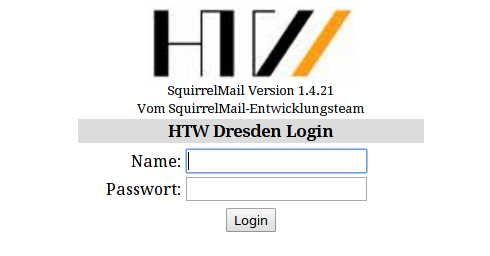
\includegraphics[width=0.7\textwidth]{../images/wm_loginseite.png}
   \end{figure}
}

\frame{
	\frametitle{SquirrelMail Startseite}
	Nach dem Login erh\"alt man eine \"Ubersicht der empfangen Mails und kann im oberen Bereich folgende Funktionen w\"ahlen:
	\begin{description}
		\item[Verfassen] E-Mail schreiben
		\item[Adressen]
		\item[Ordner] erstellen/umbenennen/l\"oschen/austragen der eintragen
		\item[Optionen] Manage Identities/Farbthema
		\item[Suchen]
		\item[Hilfe]
		\item[Filter] Filterregeln (de)aktivieren/erstellen
		\item[Kalender]
	\end{description}
	}
\frame{
	\frametitle{SquirrelMail Startseite II}
   \begin{figure}
	   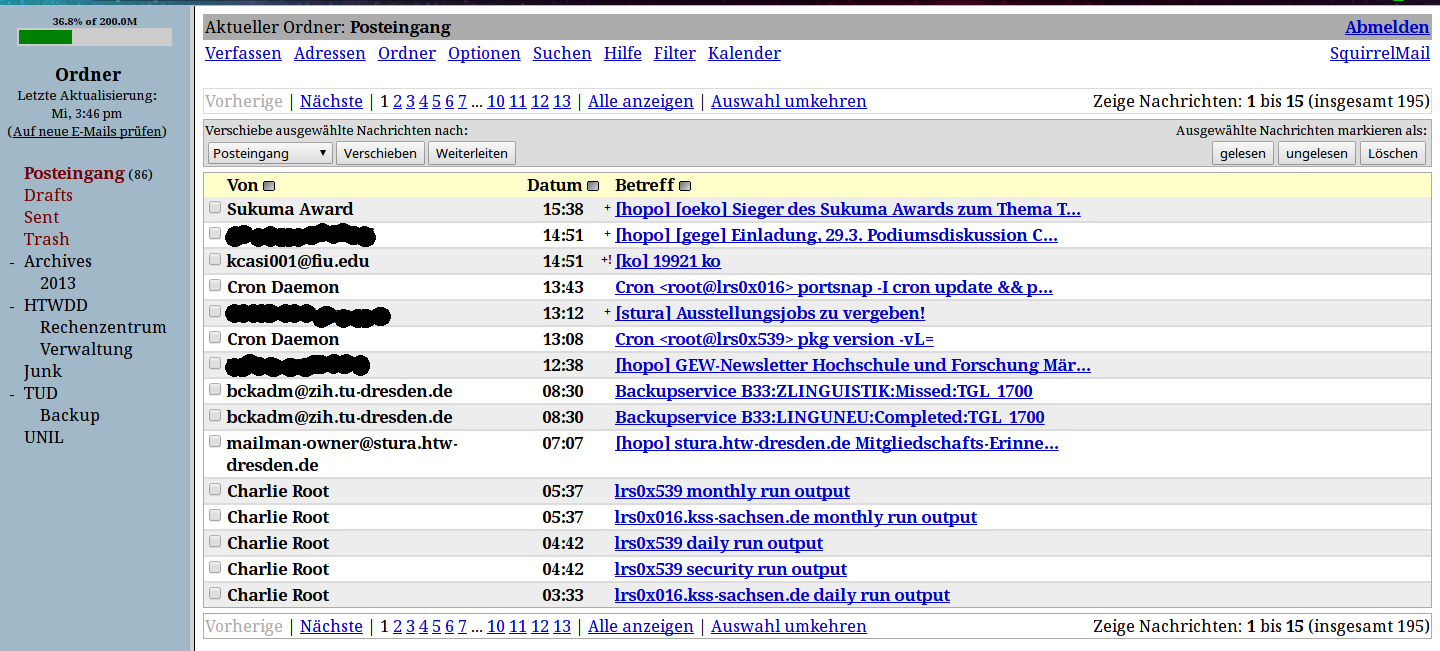
\includegraphics[width=\textwidth]{../images/wm_startseite.png}
   \end{figure}
}
\subsecframe{Ordner}{
	\begin{itemize}
		\item erstellen
		\item umbenennen
		\item l\"oschen
		\item austragen/eintragen
	\end{itemize}
	}
\frame{
	\frametitle{Ordner II}
   \begin{figure}
	   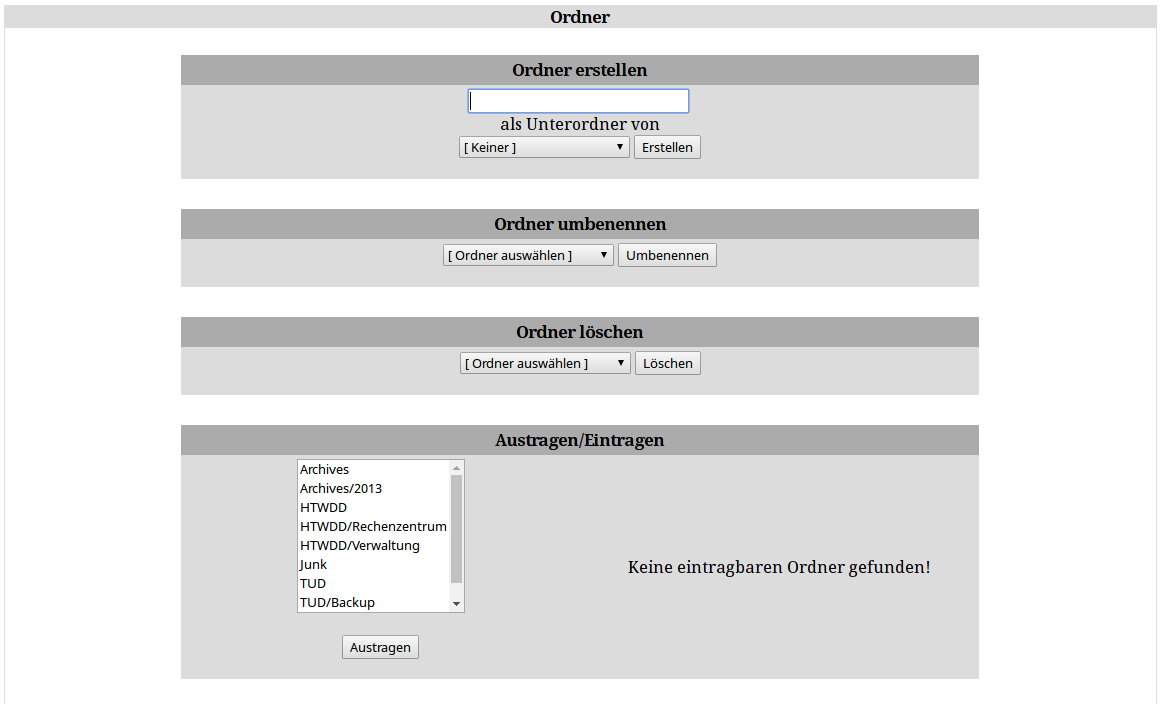
\includegraphics[width=\textwidth]{../images/wm_ordner.png}
   \end{figure}
}

\subsecframe{Optionen}{
	Manage Identities / Aliases
	}

\subsecframe{Filter} {
	\begin{itemize}
		\item aktivieren
		\item deaktivieren
		\item hinzuf\"ugen
		\item bearbeiten/kopieren/l\"oschen
	\end{itemize}
   \begin{figure}
	   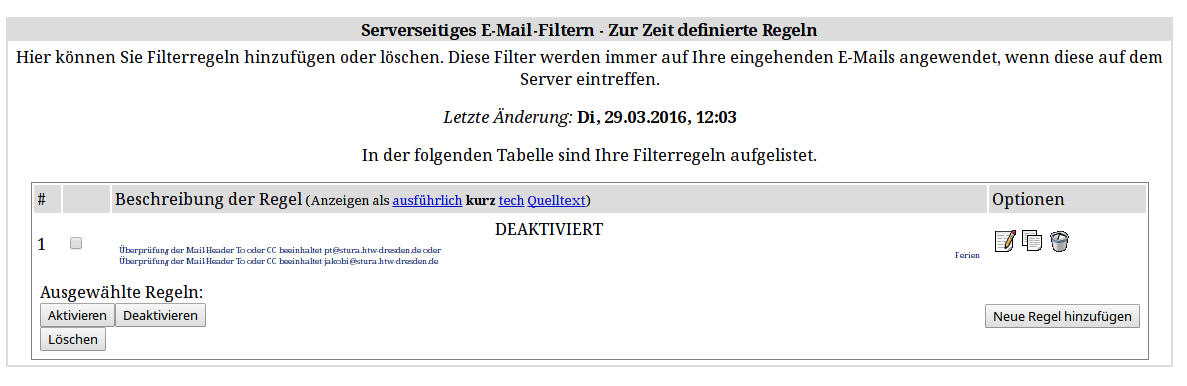
\includegraphics[width=\textwidth]{../images/wm_filterseite.png}
   \end{figure}
}

\frame{
	\frametitle{Filter II}
   \begin{figure}
	   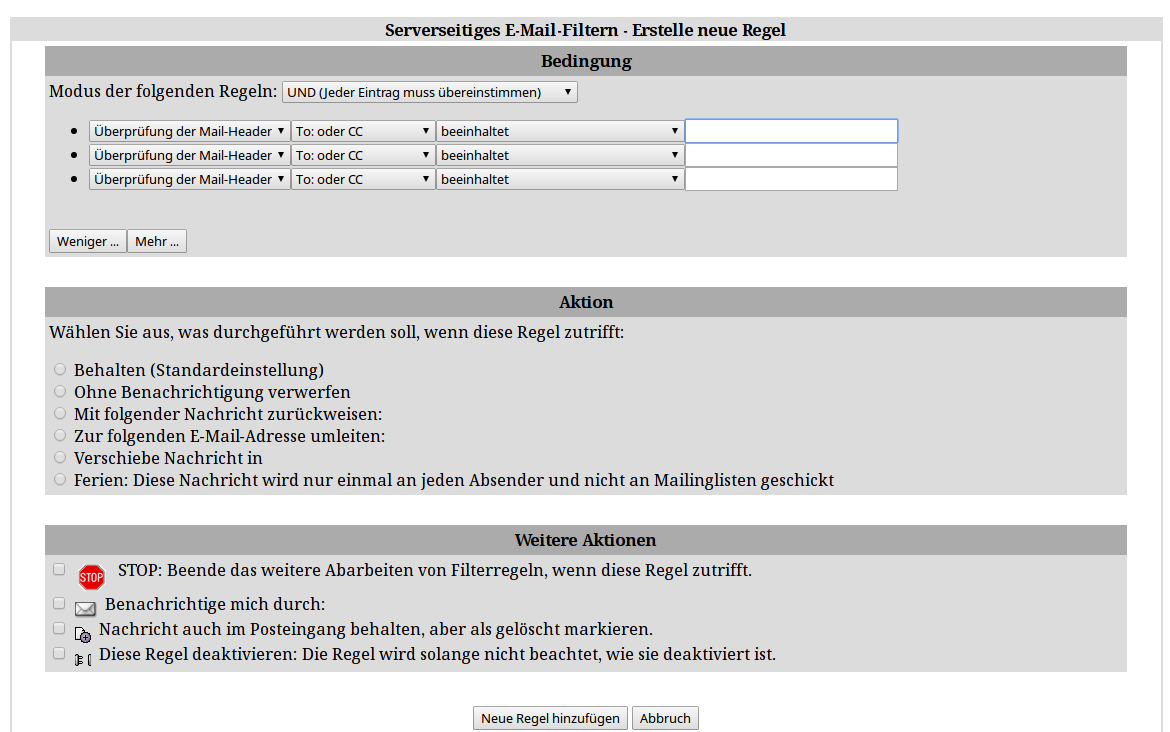
\includegraphics[width=\textwidth]{../images/wm_neue_filter_regeln.png}
   \end{figure}
}

%Webmailer
%%%webmailer url
